\documentclass[hyperref={bookmarks=false},aspectratio=169]{beamer}
\usepackage{hyperref,ragged2e,amsmath,amssymb,url,bm}
\usepackage{graphicx,booktabs,array}
\usepackage{tikz}
\usetikzlibrary{shadows}
\usetikzlibrary{arrows.meta,positioning,calc,shapes.geometric,decorations.pathreplacing,matrix}
\graphicspath{{crops/}}
\usetheme{Goettingen}
% --- Paleta "Israel": celeste y azul del tejelet (Nm 15:38), oro del santuario, fondo crema ---
% (los nombres de color se conservan por compatibilidad con los cuerpos de las láminas: «ladrillo» = azul tejelet,
%  «cafe» = azul real, «cafeosc» = azul noche, «piedra» = celeste claro, «sepia» = azul pizarra)
\definecolor{cafe}{RGB}{26,82,150}
\definecolor{cafeosc}{RGB}{11,33,74}
\definecolor{tinta}{RGB}{20,32,56}
\definecolor{oro}{RGB}{206,162,52}
\definecolor{ladrillo}{RGB}{20,68,140}
\definecolor{piedra}{RGB}{234,243,251}
\definecolor{sepia}{RGB}{72,102,140}
\definecolor{celeste}{RGB}{96,166,222}
\setbeamercolor{structure}{fg=ladrillo}
\setbeamertemplate{sidebar canvas right}[vertical shading][top=celeste!75!ladrillo,middle=ladrillo,bottom=cafeosc]
\setbeamercolor{title in sidebar}{fg=oro!80!white}
\setbeamercolor{author in sidebar}{fg=piedra}
\setbeamercolor{section in sidebar}{fg=white}
\setbeamercolor{section in sidebar shaded}{fg=celeste!45!white}
\setbeamercolor{subsection in sidebar}{fg=white}
\setbeamercolor{subsection in sidebar shaded}{fg=celeste!45!white}
\let\raggedright\justifying
\definecolor{crema}{RGB}{250,245,230}
\setbeamertemplate{background canvas}[default]
\setbeamercolor{background canvas}{bg=crema}
\setbeamercolor{normal text}{fg=tinta}
\setbeamercolor{frametitle}{fg=ladrillo}
\setbeamerfont{frametitle}{series=\bfseries}
\setbeamertemplate{section in toc shaded}{\leavevmode{\color{sepia!85!black}\inserttocsection}\par}
\setbeamercolor{title}{fg=ladrillo}
\setbeamercolor{subtitle}{fg=cafe}
\setbeamercolor{item projected}{bg=cafe,fg=piedra}
\setbeamertemplate{itemize item}{\small\textcolor{oro!85!ladrillo}{$\blacktriangleright$}}
\setbeamertemplate{navigation symbols}{}
% --- Español + hebreo + griego (XeLaTeX) con fuentes empaquetadas en fonts/ ---
\usepackage[bidi=default]{babel}
\babelprovide[import,main]{spanish}
\babelprovide[import]{hebrew}
\babelprovide[import]{ancientgreek}
\babelfont[hebrew]{sf}[Path=fonts/, BoldFont=NotoHebrewSans-700.ttf]{NotoHebrewSans-400.ttf}
\babelfont[hebrew]{rm}[Path=fonts/, BoldFont=NotoHebrewSans-700.ttf]{NotoHebrewSans-400.ttf}
\babelfont[ancientgreek]{sf}[Path=fonts/]{GFSPorson.otf}
\babelfont[ancientgreek]{rm}[Path=fonts/]{GFSPorson.otf}
\newcommand{\heb}[1]{\mbox{\foreignlanguage{hebrew}{#1}}}
\newcommand{\grc}[1]{\foreignlanguage{ancientgreek}{#1}}
% --- Citas, imágenes, referencias ---
\usepackage[most]{tcolorbox}
\newtcolorbox{cita}[1][]{enhanced, colback=piedra!92!white, colframe=oro!90!ladrillo,
  boxrule=0pt, leftrule=2.5pt, arc=0pt, left=6pt, right=6pt, top=4pt, bottom=4pt,
  before skip=4pt, after skip=6pt, fontupper=\small\itshape, #1}
\newcommand{\fuente}[1]{\par\hfill{\upshape\bfseries\footnotesize\textcolor{ladrillo}{#1}}}
\newcommand{\imagen}[3][0.80]{%
  \centering\includegraphics[height=#1\textheight,width=\linewidth,keepaspectratio]{#2}\par\vspace{2pt}
  {\fontsize{5}{6}\selectfont\color{sepia}{\raggedleft\textit{Nota.} #3\par}}}
\makeatletter
\newcommand{\fotolado}[2]{%
  % Panel a la derecha, separado de la columna de texto (0.57): marco dorado, sombra y nota al pie.
  \begin{tikzpicture}[remember picture,overlay]
    \coordinate (fl) at ([xshift=\beamer@leftmargin+0.615\textwidth]current page.west);
    \coordinate (fr) at ([xshift=-\beamer@sidebarwidth-6pt]current page.east);
    \node[inner sep=0pt,anchor=center,draw=oro,line width=0.9pt,
      drop shadow={shadow xshift=1.2pt,shadow yshift=-1.2pt,opacity=0.30,fill=cafeosc}] (foto)
      at ([yshift=6pt]$(fl)!0.5!(fr)$)
      {\includegraphics[width=\dimexpr\paperwidth-\beamer@sidebarwidth-\beamer@leftmargin-0.615\textwidth-6pt\relax]{#1}};
    \node[anchor=north east,inner sep=0pt,text=sepia,font=\fontsize{4.6}{5.6}\selectfont,align=right,
      text width=\dimexpr\paperwidth-\beamer@sidebarwidth-\beamer@leftmargin-0.615\textwidth-6pt\relax]
      at ([yshift=-3pt]foto.south east) {\textit{Nota.} #2};
  \end{tikzpicture}}
\makeatother
\newcommand{\refapa}[1]{\par\hangindent=1.2em\hangafter=1\noindent #1\par\vspace{3pt}}
\usepackage{xurl}\urlstyle{same}
\newcommand{\destacar}[1]{\textbf{\textcolor{ladrillo}{#1}}}
% --- Piezas visuales de la serie: regla dorada bajo el título, notas y pies de figura ---
\addtobeamertemplate{frametitle}{}{\vspace{-3pt}{\color{oro}\rule{2.2cm}{1.1pt}}\vspace{1pt}}
\newtcolorbox{notalam}[1][Nota]{enhanced,colback=oro!10!white,colframe=oro!85!ladrillo,boxrule=0.5pt,arc=2pt,
  left=5pt,right=5pt,top=3pt,bottom=3pt,fonttitle=\bfseries\scriptsize,coltitle=cafeosc,colbacktitle=oro!30!white,
  fontupper=\scriptsize,title={#1},before skip=4pt,after skip=4pt}
\newtcolorbox{clave}[1][]{enhanced,colback=piedra,colframe=ladrillo,boxrule=0pt,leftrule=2.5pt,arc=0pt,
  left=5pt,right=5pt,top=3pt,bottom=3pt,fontupper=\scriptsize,before skip=4pt,after skip=4pt,#1}
\newcommand{\notafig}[1]{\par\vspace{2pt}{\fontsize{5}{6}\selectfont\color{sepia}\hfill\textit{Nota.} #1\par}}
\newcommand{\elabpropia}{\notafig{Elaboración propia.}}
\tikzset{hito/.style={circle,fill=oro,draw=white,line width=0.6pt,inner sep=1.6pt},
  etiq/.style={font=\tiny,text=tinta,align=center},
  flecha/.style={->,draw=oro!90!ladrillo,line width=1pt},
  bloque/.style={draw=ladrillo,line width=0.6pt,fill=piedra,rounded corners=3pt,font=\scriptsize,align=center,inner sep=4pt},
  bloqueoro/.style={draw=oro!90!ladrillo,line width=0.6pt,fill=oro!14!white,rounded corners=3pt,font=\scriptsize,align=center,inner sep=4pt},
  bloqueazul/.style={draw=cafeosc,fill=ladrillo,text=white,rounded corners=3pt,font=\scriptsize\bfseries,align=center,inner sep=4pt}}

\tikzset{caja/.style={draw=cafe!80!black,line width=0.7pt,top color=piedra!55!white,bottom color=piedra!92!oro,
  rounded corners=4pt,inner sep=5pt,font=\scriptsize,
  drop shadow={shadow xshift=0.7pt,shadow yshift=-0.8pt,opacity=0.25,fill=cafeosc}},
  >={Stealth[length=2.4mm,width=1.8mm]}, every picture/.style={line cap=round,line join=round}}
\tikzset{invisible/.style={opacity=0,text opacity=0},visible on/.style={alt={#1{}{invisible}}},alt/.code args={<#1>#2#3}{\alt<#1>{\pgfkeysalso{#2}}{\pgfkeysalso{#3}}}}
\newcommand{\precision}[1]{{\footnotesize\color{sepia}\textbf{Precisión:} #1}}
\newcommand{\pt}[2]{({#1-30},{#2-29})}
\title[Israel 1: Abraham--Éxodo]{\bfseries{Israel, el pueblo de Dios}}
\subtitle{Estudio 1. De Abraham al Éxodo}
\author{}\institute{}\date{}
\titlegraphic{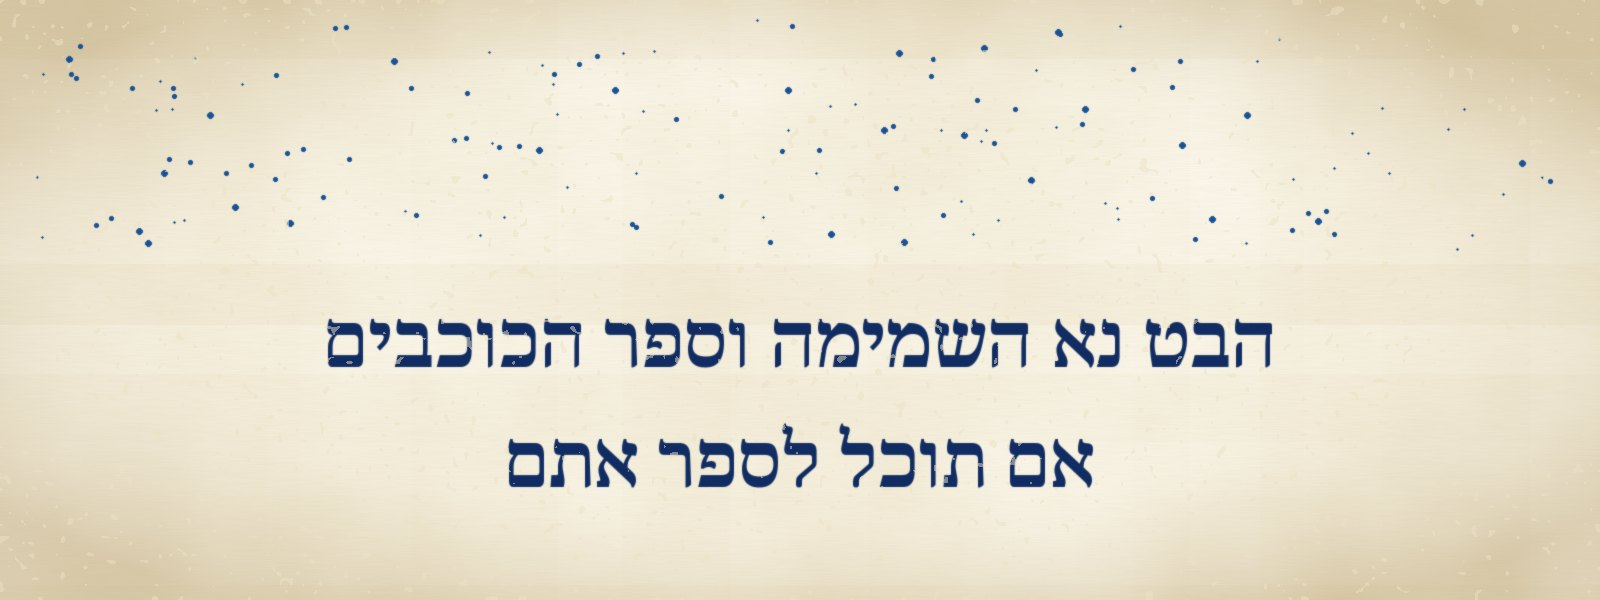
\includegraphics[width=0.85\linewidth,height=0.38\textheight,keepaspectratio]{portada.jpg}\\[-1pt]
  {\fontsize{5}{6}\selectfont\color{sepia}\textit{Nota.} Elaboración propia: Gn 15:5 en texto hebreo consonántico (BHS).}}
\begin{document}
\frame{\titlepage}

% ===================================================
\section{Introducción}
\begin{frame}{¿Por qué un pueblo?}
\begin{columns}[T,onlytextwidth]
\begin{column}{0.50\textwidth}
\begin{cita}Son israelitas; de ellos son la adopción, la gloria, los pactos, la promulgación de la ley, el culto y las promesas; de ellos son los padres, y de ellos, según la carne, vino el Mesías.\fuente{(Ro 9:4--5)}\end{cita}
\begin{cita}Porque irrevocables son los dones y el llamamiento de Dios.\fuente{(Ro 11:29)}\end{cita}
\end{column}
\begin{column}{0.46\textwidth}\small
Para entender a Pablo hay que volver al principio.\par\medskip
\centering
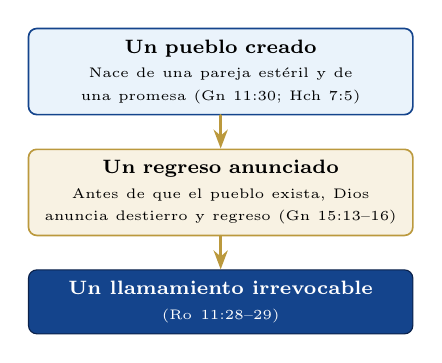
\begin{tikzpicture}[node distance=0.42cm]
\node[bloque,text width=4.6cm] (a) {\textbf{Un pueblo creado}\\[1pt]{\tiny Nace de una pareja estéril y de una promesa (Gn 11:30; Hch 7:5)}};
\begin{scope}[visible on=<2->]\node[bloqueoro,text width=4.6cm,below=of a] (b) {\textbf{Un regreso anunciado}\\[1pt]{\tiny Antes de que el pueblo exista, Dios anuncia destierro y regreso (Gn 15:13--16)}};\end{scope}
\begin{scope}[visible on=<3->]\node[bloqueazul,text width=4.6cm,below=of b] (c) {Un llamamiento irrevocable\\[1pt]{\tiny\mdseries (Ro 11:28--29)}};\end{scope}
\begin{scope}[visible on=<3->]\draw[flecha] (a) -- (b);\end{scope} \begin{scope}[visible on=<3->]\draw[flecha] (b) -- (c);\end{scope}
\end{tikzpicture}
\elabpropia
\end{column}
\end{columns}
\end{frame}

\begin{frame}{Los ejes de la serie en esta etapa}
\centering
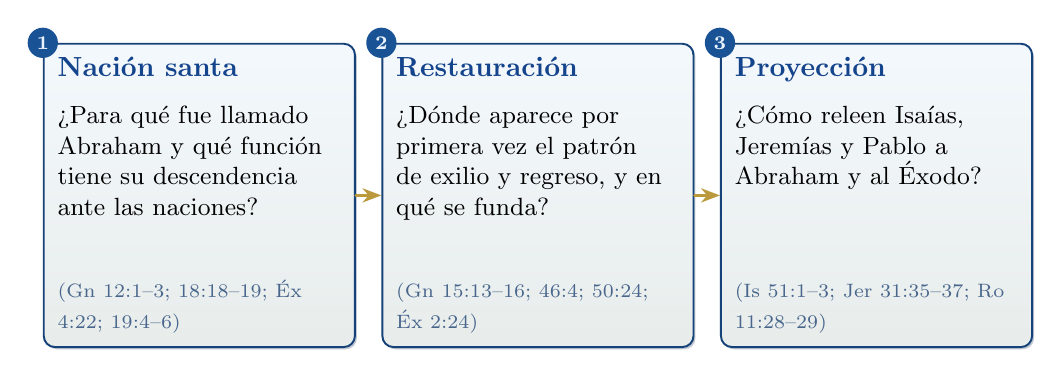
\begin{tikzpicture}
 \foreach \x/\n/\t/\d/\r [count=\ovc,evaluate=\ovc as \ovk using int(\ovc+0)] in {0/1/{Nación santa}/{¿Para qué fue llamado Abraham y qué función tiene su descendencia ante las naciones?}/{Gn 12:1--3; 18:18--19; Éx 4:22; 19:4--6},
   4.3/2/{Restauración}/{¿Dónde aparece por primera vez el patrón de exilio y regreso, y en qué se funda?}/{Gn 15:13--16; 46:4; 50:24; Éx 2:24},
   8.6/3/{Proyección}/{¿Cómo releen Isaías, Jeremías y Pablo a Abraham y al Éxodo?}/{Is 51:1--3; Jer 31:35--37; Ro 11:28--29}}{\begin{scope}[visible on=<\ovk->]
  \node[caja,anchor=north] (b\n) at (\x,0) {\parbox[t][3.5cm][t]{3.6cm}{\RaggedRight
    {\normalsize\textbf{\textcolor{ladrillo}{\t}}}\\[6pt]\small \d\par\vfill{\scriptsize\color{sepia}(\r)}}};
  \node[circle,fill=cafe,text=piedra,font=\scriptsize\bfseries,inner sep=1.6pt] at (b\n.north west) {\n};\end{scope}}
\begin{scope}[visible on=<3->]\draw[flecha] (b1.east) -- (b2.west);\end{scope} \begin{scope}[visible on=<3->]\draw[flecha] (b2.east) -- (b3.west);\end{scope}
\end{tikzpicture}
\elabpropia
\vspace{4pt}
\begin{notalam}[Sobre traducción y numeración]
Las citas bíblicas son traducción propia desde el texto hebreo (BHS) y griego (NA28); la Septuaginta se cita según Rahlfs-Hanhart. Cuando la numeración hebrea difiere de la española, se da la española y la hebrea entre corchetes: Gn 32:28 [32:29].
\end{notalam}
\end{frame}

% ===================================================
\section{Cronología}
\begin{frame}{Secuencia de la etapa}
\centering\vspace*{6pt}
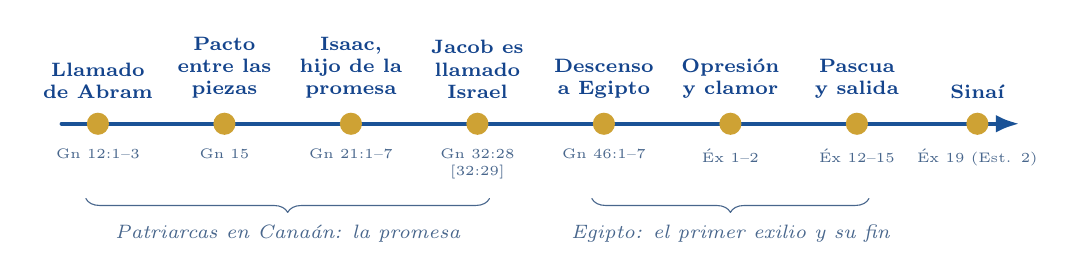
\begin{tikzpicture}[x=0.765cm]
\draw[line width=1.6pt,cafe,-{Latex[length=3mm]}] (0,0) -- (15.9,0);
\foreach \x/\t/\b [count=\ovc,evaluate=\ovc as \ovk using int(\ovc+0)] in {0.6/{Llamado de Abram}/{Gn 12:1--3},
                      2.7/{Pacto entre las piezas}/{Gn 15},
                      4.8/{Isaac, hijo de la promesa}/{Gn 21:1--7},
                      6.9/{Jacob es llamado Israel}/{Gn 32:28 [32:29]},
                      9.0/{Descenso a Egipto}/{Gn 46:1--7},
                      11.1/{Opresión y clamor}/{Éx 1--2},
                      13.2/{Pascua y salida}/{Éx 12--15},
                      15.2/{Sinaí}/{Éx 19 (Est. 2)}}{\begin{scope}[visible on=<\ovk->]
  \fill[oro] (\x,0) circle (4pt);
  \node[above,font=\scriptsize\bfseries,text=ladrillo,text width=1.55cm,align=center] at (\x,0.2) {\t};
  \node[below,font=\tiny,text=sepia,text width=1.55cm,align=center] at (\x,-0.2) {\b};\end{scope}}
\begin{scope}[visible on=<8->]\draw[decorate,decoration={brace,amplitude=5pt,mirror},sepia] (0.4,-0.95) -- (7.1,-0.95) node[midway,below=6pt,font=\scriptsize\itshape]{Patriarcas en Canaán: la promesa};\end{scope}
\begin{scope}[visible on=<8->]\draw[decorate,decoration={brace,amplitude=5pt,mirror},sepia] (8.8,-0.95) -- (13.4,-0.95) node[midway,below=6pt,font=\scriptsize\itshape]{Egipto: el primer exilio y su fin};\end{scope}
\end{tikzpicture}
\notafig{Elaboración propia. Secuencia narrativa; las fechas absolutas están en debate.}
\vspace{8pt}
\begin{clave}
La promesa precede al pueblo: el destierro en Egipto y el regreso ya están anunciados en Gn 15, antes del nacimiento de Isaac.
\end{clave}
\end{frame}

\begin{frame}{¿Cuándo fue el Éxodo?}
\begin{columns}[T,onlytextwidth]
\begin{column}{0.55\textwidth}
\centering
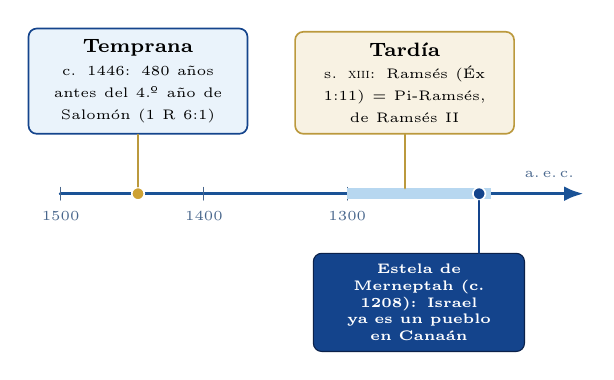
\begin{tikzpicture}[x=0.0182cm]
% eje: 1500 a 1150 a.e.c. (x = 1500 - año)
\draw[line width=1.3pt,cafe,-{Latex[length=2.5mm]}] (0,0) -- (365,0);
\foreach \a in {1500,1400,1300}{\draw[sepia] ({1500-\a},-0.08) -- ({1500-\a},0.08);
  \node[font=\tiny,text=sepia,below] at ({1500-\a},-0.1) {\a};}
\node[font=\tiny,text=sepia,anchor=south east] at (365,0.08) {a.\,e.\,c.};
% temprana
\begin{scope}[visible on=<2->]\node[hito] (t) at (54,0) {};\end{scope}
\begin{scope}[visible on=<3->]\node[bloque,text width=2.5cm,anchor=south] (tt) at (54,0.75) {\textbf{Temprana}\\{\tiny c. 1446: 480 años antes del 4.º año de Salomón (1~R 6:1)}};\end{scope}
\begin{scope}[visible on=<3->]\draw[oro!90!ladrillo,line width=0.8pt] (tt.south) -- (t);\end{scope}
% tardía
\begin{scope}[visible on=<4->]\fill[celeste!45] (200,-0.07) rectangle (300,0.07);\end{scope}
\begin{scope}[visible on=<4->]\node[bloqueoro,text width=2.5cm,anchor=south] (dd) at (240,0.75) {\textbf{Tardía}\\{\tiny s. \textsc{xiii}: Ramsés (Éx 1:11) = Pi-Ramsés, de Ramsés~II}};\end{scope}
\begin{scope}[visible on=<4->]\draw[oro!90!ladrillo,line width=0.8pt] (dd.south) -- (240,0.07);\end{scope}
% Merneptah
\begin{scope}[visible on=<5->]\node[hito,fill=ladrillo] (m) at (292,0) {};\end{scope}
\begin{scope}[visible on=<6->]\node[bloqueazul,text width=2.4cm,anchor=north,font=\tiny\bfseries] (mm) at (250,-0.75) {Estela de Merneptah (c. 1208): Israel ya es un pueblo en Canaán};\end{scope}
\begin{scope}[visible on=<6->]\draw[ladrillo,line width=0.8pt] (m) -- (m|-mm.north);\end{scope}
\end{tikzpicture}
\notafig{Elaboración propia a partir de Hoffmeier (1997) y Kitchen (2003).}
\end{column}
\begin{column}{0.42\textwidth}
\begin{notalam}[Un argumento de la fecha temprana]
El nombre «Ramsés» pudo actualizarse durante la transmisión del texto, como ocurre con «Dan» en Gn 14:14, ciudad que recibió ese nombre mucho después de Abraham.
\end{notalam}
\begin{clave}
El debate sigue abierto. Para el argumento basta la secuencia de los hechos, no el año exacto.
\end{clave}
\end{column}
\end{columns}
\end{frame}

\begin{frame}{Los 430 años de Éx 12:40}
\begin{columns}[T,onlytextwidth]
\begin{column}{0.56\textwidth}
\footnotesize\renewcommand{\arraystretch}{1.25}
\begin{tabular}{>{\RaggedRight\arraybackslash}p{2.3cm}>{\RaggedRight\arraybackslash}p{4.05cm}}
\toprule
{\leavevmode\color{ladrillo}\bfseries Fuente} & {\leavevmode\color{ladrillo}\bfseries Lectura}\\\midrule
Texto Masorético & 430 años en Egipto\\
LXX y Pentateuco samaritano & 430 años «en Egipto \emph{y en Canaán}»\\
Pablo (Gá 3:17) & 430 años de la promesa a la ley\\
Josefo (\emph{Ant.} 2.15.2) & 215 años en Egipto\\
Seder Olam; Rashi & 400 años desde Isaac; c. 210 en Egipto\\
\bottomrule
\end{tabular}
\notafig{Elaboración propia a partir de Guggenheimer (1998) y Josefo (1987).}
\end{column}
\begin{column}{0.40\textwidth}
\begin{notalam}[Precisión textual]
El TM cuenta 430 años de permanencia en Egipto. La cronología rabínica cuenta los 400 años de Gn 15:13 desde el nacimiento de Isaac (Seder Olam Rabbah). Este estudio sigue el TM y señala la lectura alternativa.
\end{notalam}
\end{column}
\end{columns}
\end{frame}

% ===================================================
\section{Arqueología}
\begin{frame}{El camino de Abraham}
\begin{columns}[c,onlytextwidth]
\begin{column}{0.64\textwidth}\centering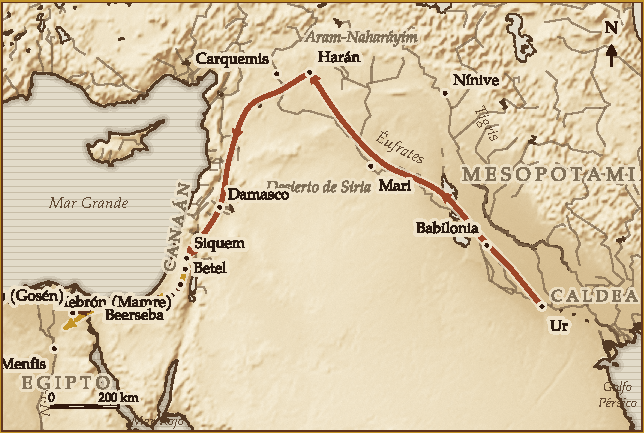
\includegraphics[width=\linewidth,height=0.84\textheight,keepaspectratio]{mapa_patriarcas.pdf}
\notafig{Elaboración propia (GSHHS/WDB, Basemap); ubicaciones aproximadas.}\end{column}
\begin{column}{0.33\textwidth}\scriptsize\RaggedRight
{\scriptsize\RaggedRight
\tikz[baseline=-0.6ex]\draw[ladrillo,line width=1.5pt,line cap=round](0,0)--(0.6,0);~Taré y Abram: Ur $\to$ Harán (Gn 11:31)\par
\tikz[baseline=-0.6ex]\draw[ladrillo,line width=1.5pt,line cap=round](0,0)--(0.6,0);~Abram: Harán $\to$ Siquem (Gn 12:4–6)\par
\tikz[baseline=-0.6ex]\draw[oro,line width=1.5pt,line cap=round,dash pattern=on 3.4pt off 1.8pt](0,0)--(0.6,0);~Abram a Egipto (Gn 12:10)\par
\tikz[baseline=-0.6ex]\draw[cafe,line width=1.5pt,line cap=round,dash pattern=on 1.2pt off 1.4pt](0,0)--(0.6,0);~Jacob y su casa a Egipto (Gn 46)\par}

\end{column}
\end{columns}
\end{frame}

\begin{frame}{Ur, Harán, Siquem: dejar tierra y dioses}
\centering
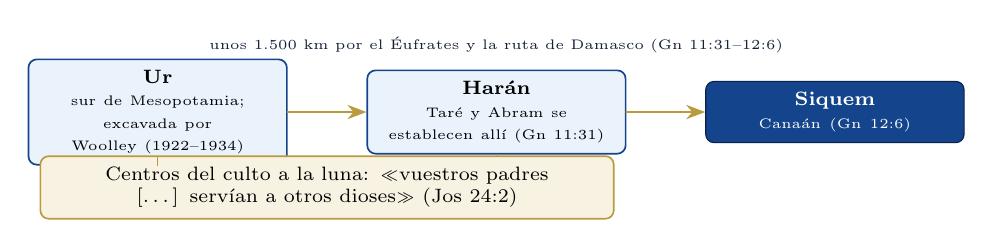
\begin{tikzpicture}[node distance=1.0cm]
\node[bloque,text width=3.0cm] (u) {\textbf{Ur}\\{\tiny sur de Mesopotamia; excavada por Woolley (1922--1934)}};
\begin{scope}[visible on=<2->]\node[bloque,text width=3.0cm,right=of u] (h) {\textbf{Harán}\\{\tiny Taré y Abram se establecen allí (Gn 11:31)}};\end{scope}
\begin{scope}[visible on=<3->]\node[bloqueazul,text width=3.0cm,right=of h] (s) {Siquem\\{\tiny\mdseries Canaán (Gn 12:6)}};\end{scope}
\begin{scope}[visible on=<3->]\draw[flecha] (u) -- (h);\end{scope} \begin{scope}[visible on=<3->]\draw[flecha] (h) -- (s);\end{scope}
\begin{scope}[visible on=<4->]\node[bloqueoro,text width=7.0cm,below=0.55cm of $(u)!0.5!(h)$] (c) {Centros del culto a la luna: «vuestros padres [\ldots] servían a otros dioses» (Jos 24:2)};\end{scope}
\begin{scope}[visible on=<4->]\draw[oro!90!ladrillo,dashed] (u.south) -- (u.south|-c.north);\end{scope} \begin{scope}[visible on=<4->]\draw[oro!90!ladrillo,dashed] (h.south) -- (h.south|-c.north);\end{scope}
\begin{scope}[visible on=<5->]\node[etiq,above=2pt of $(u)!0.5!(s)$,yshift=0.55cm] {unos 1.500 km por el Éufrates y la ruta de Damasco (Gn 11:31--12:6)};\end{scope}
\end{tikzpicture}
\elabpropia
\vspace{6pt}
\begin{columns}[T,onlytextwidth]
\begin{column}{0.48\textwidth}
\begin{notalam}[¿Qué Ur?]
«De los caldeos» refleja una denominación posterior; una tradición antigua sitúa Ur en Urfa, cerca de Harán (Sarna, 1989).
\end{notalam}
\end{column}
\begin{column}{0.48\textwidth}
\begin{clave}
Canaán es el puente entre los dos imperios fluviales, Egipto y Mesopotamia: camino de Abram, de Jacob y de todo Israel.
\end{clave}
\end{column}
\end{columns}
\end{frame}

\begin{frame}{Semitas en Egipto}
\centering
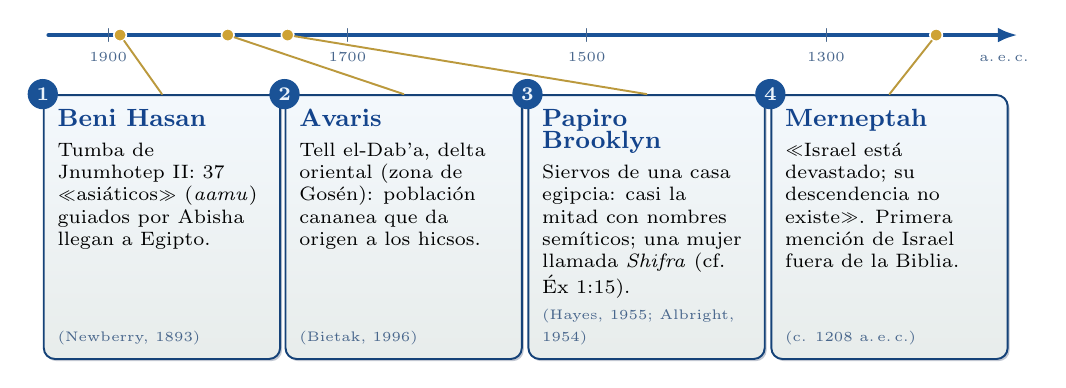
\begin{tikzpicture}[x=0.0152cm]
% eje: 1950 a 1150 a.e.c. (x = 1950 - año)
\draw[line width=1.3pt,cafe,-{Latex[length=2.5mm]}] (0,0) -- (810,0);
\foreach \a in {1900,1700,1500,1300}{\draw[sepia] ({1950-\a},-0.08) -- ({1950-\a},0.08);
  \node[font=\tiny,text=sepia,below] at ({1950-\a},-0.1) {\a};}
\node[font=\tiny,text=sepia,anchor=west] at (770,-0.30) {a.\,e.\,c.};
\foreach \a/\n/\px/\t/\d/\r [count=\ovc,evaluate=\ovc as \ovk using int(\ovc+0)] in {1890/1/95/{Beni Hasan}/{Tumba de Jnumhotep~II: 37 «asiáticos» (\emph{aamu}) guiados por Abisha llegan a Egipto.}/{Newberry, 1893},
   1800/2/297/{Avaris}/{Tell el-Dab\textquoteright a, delta oriental (zona de Gosén): población cananea que da origen a los hicsos.}/{Bietak, 1996},
   1750/3/500/{Papiro Brooklyn}/{Siervos de una casa egipcia: casi la mitad con nombres semíticos; una mujer llamada \emph{Shifra} (cf. Éx 1:15).}/{Hayes, 1955; Albright, 1954},
   1208/4/703/{Merneptah}/{«Israel está devastado; su descendencia no existe». Primera mención de Israel fuera de la Biblia.}/{c. 1208 a.\,e.\,c.}}{\begin{scope}[visible on=<\ovk->]
  \node[hito] (p\n) at ({1950-\a},0) {};
  \node[caja,anchor=north] (b\n) at (\px,-0.75) {\parbox[t][3.0cm][t]{2.65cm}{\RaggedRight
    {\small\textbf{\textcolor{ladrillo}{\t}}}\\[3pt]\scriptsize \d\par\vfill{\tiny\color{sepia}(\r)}}};
  \draw[oro!90!ladrillo,line width=0.7pt] (p\n) -- (b\n.north);
  \node[circle,fill=cafe,text=piedra,font=\scriptsize\bfseries,inner sep=1.6pt] at (b\n.north west) {\n};\end{scope}}
\end{tikzpicture}
\notafig{Elaboración propia. Fechas aproximadas; el Papiro Brooklyn data de fines del Reino Medio.}
\vspace{4pt}
\begin{clave}
Ninguno nombra a José ni a Jacob; juntos, hacen verosímil el mundo que describe Génesis.
\end{clave}
\end{frame}

\begin{frame}{Lo que la arqueología no dice}
\centering
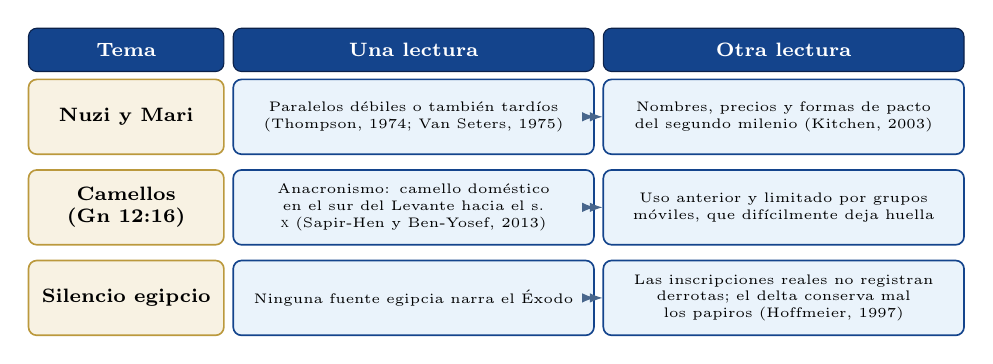
\begin{tikzpicture}
\node[bloqueazul,text width=2.2cm,minimum height=0.55cm] at (0,0.85) {Tema};
\node[bloqueazul,text width=4.3cm,minimum height=0.55cm] at (3.65,0.85) {Una lectura};
\node[bloqueazul,text width=4.3cm,minimum height=0.55cm] at (8.35,0.85) {Otra lectura};
\foreach \y/\t/\a/\b [count=\ovc,evaluate=\ovc as \ovk using int(\ovc+0)] in {0/{Nuzi y Mari}/{Paralelos débiles o también tardíos (Thompson, 1974; Van Seters, 1975)}/{Nombres, precios y formas de pacto del segundo milenio (Kitchen, 2003)},
  -1.15/{Camellos (Gn 12:16)}/{Anacronismo: camello doméstico en el sur del Levante hacia el s. \textsc{x} (Sapir-Hen y Ben-Yosef, 2013)}/{Uso anterior y limitado por grupos móviles, que difícilmente deja huella},
  -2.30/{Silencio egipcio}/{Ninguna fuente egipcia narra el Éxodo}/{Las inscripciones reales no registran derrotas; el delta conserva mal los papiros (Hoffmeier, 1997)}}{\begin{scope}[visible on=<\ovk->]
  \node[bloqueoro,text width=2.2cm,minimum height=0.95cm,font=\scriptsize\bfseries] at (0,\y) {\t};
  \node[bloque,text width=4.3cm,minimum height=0.95cm,font=\tiny] (l) at (3.65,\y) {\a};
  \node[bloque,text width=4.3cm,minimum height=0.95cm,font=\tiny] (r) at (8.35,\y) {\b};
  \draw[{Latex[length=1.6mm]}-{Latex[length=1.6mm]},sepia] (l.east) -- (r.west);\end{scope}}
\end{tikzpicture}
\elabpropia
\vspace{4pt}
\begin{notalam}[Lo que sí concuerda]
Hoffmeier (1997) observa que los nombres egipcios de Moisés, Putifar o Zafnat-panea, el trabajo con ladrillos y paja de Éx 5 y la geografía del delta oriental concuerdan con lo que se sabe de Egipto. Sin evidencia directa: cautela, pero no negación del relato.
\end{notalam}
\end{frame}

% ===================================================
\section{El relato}
\begin{frame}{Babel y Abram: dos nombres}
\centering
\begin{tikzpicture}
\node[bloqueazul,text width=4.6cm] (bh) at (0,0) {Babel (Gn 11)};
\node[bloqueazul,text width=4.6cm] (ah) at (6.6,0) {Abram (Gn 12)};
\foreach \y/\l/\r [count=\ovc,evaluate=\ovc as \ovk using int(\ovc+0)] in {-0.85/{«Hagámonos un nombre» \heb{וְנַעֲשֶׂה־לָּנוּ שֵׁם} (Gn 11:4)}/{«Engrandeceré tu nombre» (Gn 12:2)},
  -1.75/{Iniciativa humana: «hagamos»}/{Iniciativa divina: «haré», «bendeciré», «engrandeceré»},
  -2.65/{Una ciudad que se cierra sobre sí}/{Una nación (\heb{גּוֹי}, \emph{goy}) con una tarea: «sé una bendición»},
  -3.55/{Las familias quedan dispersas (Gn 11:8--9)}/{«En ti serán benditas todas las familias de la tierra» (Gn 12:3)}}{\begin{scope}[visible on=<\ovk->]
  \node[bloque,text width=4.6cm,minimum height=0.7cm] (l) at (0,\y) {\l};
  \node[bloqueoro,text width=4.6cm,minimum height=0.7cm] (r) at (6.6,\y) {\r};
  \draw[flecha] (l.east) -- (r.west);\end{scope}}
\end{tikzpicture}
\elabpropia
\vspace{6pt}
\begin{clave}
El narrador responde a la ambición de Babel con un contraste deliberado: ahora es Dios quien da nombre, y lo da para bendecir a las familias que Gn 10 enumeró y Gn 11 dispersó.
\end{clave}
\end{frame}

\begin{frame}{Un nombre recibido}
\fotolado{panel_gn12.jpg}{Elaboración propia: Gn 12:2--3 en texto hebreo consonántico (BHS).}
\begin{columns}[c,onlytextwidth]
\begin{column}{0.57\textwidth}
\begin{cita}Haré de ti una nación grande, te bendeciré y engrandeceré tu nombre, y sé tú una bendición [\ldots]; y en ti serán benditas todas las familias de la tierra.\fuente{(Gn 12:2--3)}\end{cita}
\begin{notalam}[El imperativo de la bendición]
\heb{וֶהְיֵה בְּרָכָה} (\emph{ve-heyé berajá}), «sé una bendición»: un imperativo dentro de la promesa. La nación no se agota en sí misma; recibe una tarea que mira hacia «todas las familias de la tierra».
\end{notalam}
\end{column}
\begin{column}{0.41\textwidth}\end{column}
\end{columns}
\end{frame}

\begin{frame}{«En ti serán benditas»: del hebreo a Pablo}
\centering\vspace*{4pt}
\begin{tikzpicture}[node distance=0.95cm]
\node[caja,text width=3.3cm,align=center] (h) {\textbf{Hebreo (Gn 12:3)}\\[3pt]\heb{וְנִבְרְכוּ בְךָ}\\[2pt]\emph{ve-nivrejú vejá}\\[2pt]nifal: pasivo o reflexivo};
\begin{scope}[visible on=<2->]\node[caja,text width=3.3cm,align=center,right=of h] (g) {\textbf{LXX}\\[3pt]\grc{ἐνευλογηθήσονται ἐν σοί}\\[2pt]futuro pasivo:\\«serán benditas»};\end{scope}
\begin{scope}[visible on=<3->]\node[caja,text width=3.3cm,align=center,right=of g] (p) {\textbf{Pablo (Gá 3:8)}\\[3pt]\grc{πάντα τὰ ἔθνη}\\[2pt]«todas las naciones»\\(de Gn 18:18; 22:18)};\end{scope}
\begin{scope}[visible on=<3->]\draw[-{Latex[length=2.5mm]},oro!90!ladrillo,line width=1.4pt] (h) -- (g);\end{scope}
\begin{scope}[visible on=<3->]\draw[-{Latex[length=2.5mm]},oro!90!ladrillo,line width=1.4pt] (g) -- (p);\end{scope}
\end{tikzpicture}
\elabpropia
\vspace{6pt}
{\small\itshape\color{sepia}Pablo funde Gn 12:3 con Gn 18:18 y llama a esta promesa «evangelio anunciado de antemano a Abraham».}\par\vspace{6pt}
\begin{notalam}[Precisión filológica]
Gn 22:18 y 26:4 usan el hitpael \heb{וְהִתְבָּרְכוּ}, que favorece «se bendecirán», es decir, usarán tu nombre al bendecir. Con cualquiera de las dos lecturas, el destino de las naciones queda atado a Abraham.
\end{notalam}
\end{frame}

\begin{frame}{Gn 15: la fe de Abram}
\begin{columns}[T,onlytextwidth]
\begin{column}{0.50\textwidth}
\centering\vspace*{4pt}{\large\heb{וְהֶאֱמִן בַּיהוָה וַיַּחְשְׁבֶהָ לּוֹ צְדָקָה}}\par\medskip
\begin{cita}Y creyó a YHWH, y él se lo contó por justicia.\fuente{(Gn 15:6)}\end{cita}
\begin{notalam}[\emph{He'emín}]
\heb{הֶאֱמִן}, de la raíz \emph{'mn} (\emph{amén}, \emph{emuná}): apoyarse en alguien como en algo firme.
\end{notalam}
\end{column}
\begin{column}{0.46\textwidth}
\centering
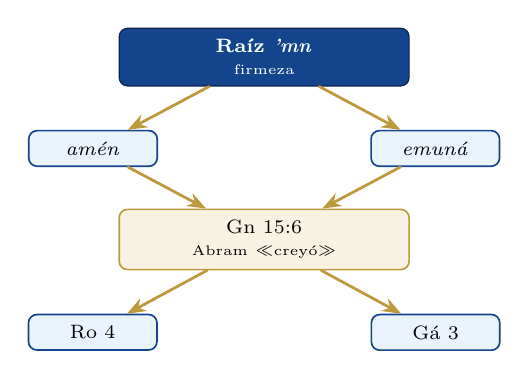
\begin{tikzpicture}[node distance=0.45cm]
\node[bloqueazul,text width=3.4cm] (r) {Raíz \emph{'mn}\\{\tiny\mdseries firmeza}};
\begin{scope}[visible on=<2->]\node[bloque,text width=1.35cm,below left=0.55cm and -0.5cm of r] (a) {\emph{amén}};\end{scope}
\begin{scope}[visible on=<3->]\node[bloque,text width=1.35cm,below right=0.55cm and -0.5cm of r] (e) {\emph{emuná}};\end{scope}
\begin{scope}[visible on=<4->]\node[bloqueoro,text width=3.4cm,below=1.55cm of r] (g) {Gn 15:6\\{\tiny Abram «creyó»}};\end{scope}
\begin{scope}[visible on=<4->]\draw[flecha] (r) -- (a);\end{scope} \begin{scope}[visible on=<4->]\draw[flecha] (r) -- (e);\end{scope}
\begin{scope}[visible on=<4->]\draw[flecha] (a) -- (g);\end{scope} \begin{scope}[visible on=<4->]\draw[flecha] (e) -- (g);\end{scope}
\begin{scope}[visible on=<5->]\node[bloque,text width=1.35cm,below left=0.55cm and -0.5cm of g] (ro) {Ro 4};\end{scope}
\begin{scope}[visible on=<6->]\node[bloque,text width=1.35cm,below right=0.55cm and -0.5cm of g] (ga) {Gá 3};\end{scope}
\begin{scope}[visible on=<6->]\draw[flecha] (g) -- (ro);\end{scope} \begin{scope}[visible on=<6->]\draw[flecha] (g) -- (ga);\end{scope}
\end{tikzpicture}
\elabpropia
\end{column}
\end{columns}
\end{frame}

\begin{frame}{El pacto entre las piezas (Gn 15:17)}
\begin{columns}[T,onlytextwidth]
\begin{column}{0.50\textwidth}
\centering
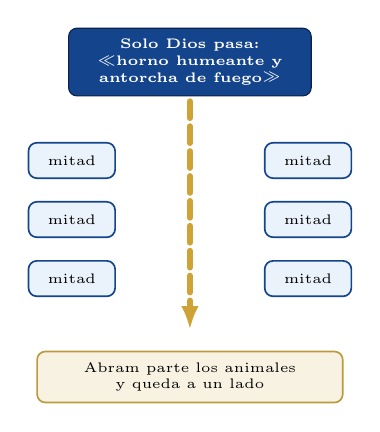
\begin{tikzpicture}
\foreach \i in {0,1,2}{
  \node[bloque,minimum width=1.1cm,minimum height=0.45cm,font=\tiny] at (0,-\i*0.75) {mitad};
  \node[bloque,minimum width=1.1cm,minimum height=0.45cm,font=\tiny] at (3.0,-\i*0.75) {mitad};}
\draw[oro,line width=2.2pt,-{Latex[length=3mm]},dash pattern=on 6pt off 3pt] (1.5,0.75) -- (1.5,-2.15);
\begin{scope}[visible on=<2->]\node[bloqueazul,text width=2.8cm,font=\tiny\bfseries] at (1.5,1.25) {Solo Dios pasa: «horno humeante y antorcha de fuego»};\end{scope}
\begin{scope}[visible on=<3->]\node[bloqueoro,text width=3.6cm,font=\tiny] at (1.5,-2.75) {Abram parte los animales y queda a un lado};\end{scope}
\end{tikzpicture}
\elabpropia
\end{column}
\begin{column}{0.46\textwidth}\small
\begin{itemize}
\item En los tratados antiguos, quien pasaba entre las mitades se maldecía a sí mismo si rompía el pacto (Jer 34:18--20).
\item Al pasar solo, \destacar{Dios carga con toda la obligación}.
\end{itemize}
\vspace{4pt}
\begin{notalam}[Tradición judía]
El pasaje se conoce como \emph{berit bein ha-betarim} (\heb{בְּרִית בֵּין הַבְּתָרִים}), «el pacto entre las piezas» (Gn 15:7--21).
\end{notalam}
\end{column}
\end{columns}
\end{frame}

\begin{frame}{El primer anuncio de exilio y regreso}
\begin{cita}Tu descendencia será extranjera en una tierra que no es suya; los harán servir y los oprimirán cuatrocientos años. Pero a la nación a la que servirán la juzgaré yo, y después saldrán con gran riqueza [\ldots]. Y en la cuarta generación \textbf{volverán} acá.\fuente{(Gn 15:13--14, 16)}\end{cita}
\centering

\begin{tikzpicture}[node distance=0.55cm]
\foreach \i/\t/\s [count=\k] in {0/Promesa/{Gn 15:5--7},1/Destierro/{15:13},2/Juicio al opresor/{15:14a},3/Regreso/{15:14b, 16}}{
  \node[caja,text width=2.3cm,align=center,minimum height=1.0cm] (n\k) at (\i*3.2,0) {\textbf{\textcolor{ladrillo}{\t}}\\[1pt]{\tiny\color{sepia}\s}};}
\foreach \a/\b in {1/2,2/3,3/4}{\draw[-{Latex[length=2.2mm]},oro!90!ladrillo,line width=1.3pt] (n\a) -- (n\b);}
\end{tikzpicture}
\elabpropia
\begin{notalam}[El verbo del regreso]
\heb{יָשׁוּבוּ} (\emph{yashuvu}), de \heb{שׁוּב} (\emph{shuv}): con este verbo se nombrarán el regreso del exilio y el arrepentimiento (\emph{teshuvá}) en Dt 30:3; Jer 29:14; 31:16--17. La restauración tiene un vocabulario antes de tener una historia.
\end{notalam}
\end{frame}

\begin{frame}{Perla filológica · el verbo del regreso, \heb{שׁוּב}}
{\footnotesize La raíz de \emph{yashuvu} une volver a la tierra y volverse a Dios; en los textos decisivos la iniciativa pasa a Dios.}\par\vspace{4pt}
\centering\scriptsize\renewcommand{\arraystretch}{1.22}
\begin{tabular}{>{\RaggedRight\arraybackslash}p{1.9cm}>{\RaggedRight\arraybackslash}p{4.3cm}>{\RaggedRight\arraybackslash}p{5.2cm}}
\toprule
{\color{ladrillo}\bfseries Texto} & {\color{ladrillo}\bfseries Hebreo} & {\color{ladrillo}\bfseries Sentido}\\\midrule
Gn 15:16 & \heb{וְדוֹר רְבִיעִי יָשׁוּבוּ הֵנָּה} & «Volverán acá»: primer anuncio de regreso\\
Dt 30:2--3 & \heb{וְשַׁבְתָּ} (v.~2); \heb{וְשָׁב יְהוָה אֱלֹהֶיךָ אֶת־שְׁבוּתְךָ} (v.~3) & Israel vuelve y Dios «hace volver su cautividad»\\
Jer 31:18 [31:17] & \heb{הֲשִׁבֵנִי וְאָשׁוּבָה} & Efraín: «hazme volver, y volveré»\\
Lm 5:21 & \heb{הֲשִׁיבֵנוּ יְהוָה אֵלֶיךָ וְנָשׁוּבָה} & Primero Dios hace volver; después el pueblo vuelve\\
Is 59:20 & \heb{וּלְשָׁבֵי פֶשַׁע בְּיַעֲקֹב} & Citado por Pablo en Ro 11:26\\
\bottomrule
\end{tabular}
\elabpropia
\vspace{4pt}
\begin{clave}\footnotesize El regreso geográfico de Gn 15 se vuelve en los profetas regreso del corazón (\emph{teshuvá}), y en Ro 11:26 es el Libertador quien «apartará de Jacob la impiedad».\end{clave}
\end{frame}

\begin{frame}{Gn 17: un pacto perpetuo}
\begin{columns}[T,onlytextwidth]
\begin{column}{0.46\textwidth}
\begin{cita}Estableceré mi pacto [\ldots] con tu descendencia después de ti, por sus generaciones, como pacto perpetuo (\upshape\heb{לִבְרִית עוֹלָם}).\fuente{(Gn 17:7)}\end{cita}
\small Abram pasa a ser Abraham: \heb{אַב־הֲמוֹן גּוֹיִם}, «padre de multitud de naciones» (Gn 17:5), versículo que Pablo cita en Ro 4:17.
\end{column}
\begin{column}{0.50\textwidth}
\centering
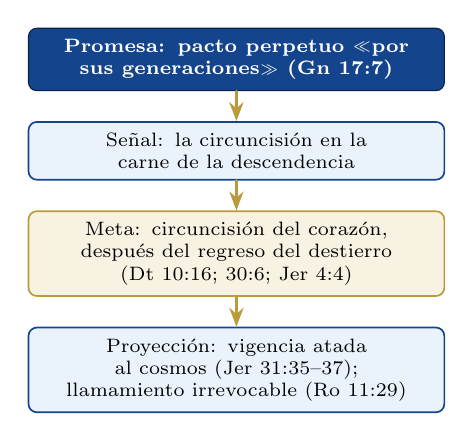
\begin{tikzpicture}[node distance=0.38cm]
\node[bloqueazul,text width=5.0cm] (p) {Promesa: pacto perpetuo «por sus generaciones» (Gn 17:7)};
\begin{scope}[visible on=<2->]\node[bloque,text width=5.0cm,below=of p] (s) {Señal: la circuncisión en la carne de la descendencia};\end{scope}
\begin{scope}[visible on=<3->]\node[bloqueoro,text width=5.0cm,below=of s] (c) {Meta: circuncisión del corazón, después del regreso del destierro (Dt 10:16; 30:6; Jer 4:4)};\end{scope}
\begin{scope}[visible on=<4->]\node[bloque,text width=5.0cm,below=of c] (i) {Proyección: vigencia atada al cosmos (Jer 31:35--37); llamamiento irrevocable (Ro 11:29)};\end{scope}
\begin{scope}[visible on=<4->]\draw[flecha] (p) -- (s);\end{scope} \begin{scope}[visible on=<4->]\draw[flecha] (s) -- (c);\end{scope} \begin{scope}[visible on=<4->]\draw[flecha] (c) -- (i);\end{scope}
\end{tikzpicture}
\elabpropia
\end{column}
\end{columns}
\end{frame}

\begin{frame}{Gn 22: la promesa entregada}
\begin{columns}[T,onlytextwidth]
\begin{column}{0.50\textwidth}\small
\begin{itemize}
\item Isaac, hijo de la imposibilidad (Gn 18:11--14), es ofrecido.
\item \heb{יְהוָה יִרְאֶה} (\emph{YHWH yiré}): «YHWH proveerá» (22:14).
\item Promesa jurada: «en tu descendencia serán benditas todas las naciones de la tierra» (22:18).
\end{itemize}
\vspace{4pt}
\begin{clave}
La promesa fue entregada y devuelta; desde entonces descansa sobre un juramento.
\end{clave}
\end{column}
\begin{column}{0.46\textwidth}
\centering
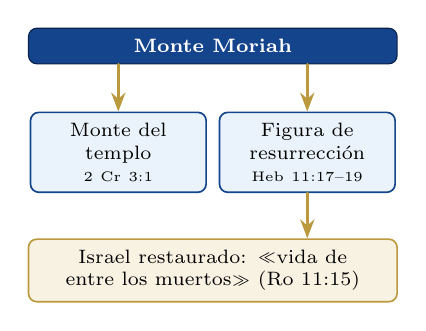
\begin{tikzpicture}
\node[bloqueazul,text width=4.4cm] (m) at (0,0) {Monte Moriah};
\begin{scope}[visible on=<2->]\node[bloque,text width=1.95cm,minimum height=0.95cm] (t) at (-1.2,-1.35) {Monte del templo\\{\tiny 2~Cr 3:1}};\end{scope}
\begin{scope}[visible on=<3->]\node[bloque,text width=1.95cm,minimum height=0.95cm] (r) at (1.2,-1.35) {Figura de resurrección\\{\tiny Heb 11:17--19}};\end{scope}
\begin{scope}[visible on=<4->]\node[bloqueoro,text width=4.4cm] (i) at (0,-2.85) {Israel restaurado: «vida de entre los muertos» (Ro 11:15)};\end{scope}
\begin{scope}[visible on=<4->]\draw[flecha] (m.south-|t) -- (t);\end{scope} \begin{scope}[visible on=<4->]\draw[flecha] (m.south-|r) -- (r);\end{scope} \begin{scope}[visible on=<4->]\draw[flecha] (r) -- (r|-i.north);\end{scope}
\end{tikzpicture}
\elabpropia
\end{column}
\end{columns}
\end{frame}

\begin{frame}{Jacob llamado Israel}
\begin{columns}[T,onlytextwidth]
\begin{column}{0.49\textwidth}
\begin{cita}No se dirá más tu nombre Jacob, sino Israel, porque has luchado con Dios y con los hombres, y has prevalecido.\fuente{(Gn 32:28 [32:29])}\end{cita}
\begin{notalam}[Etimología]
La explicación juega con \emph{sará}, «luchar»; el sentido gramatical probable es «Dios lucha» o «que Dios prevalezca» (Sarna, 1989). El pueblo lleva el nombre de un hombre herido que no soltó a Dios hasta ser bendecido.
\end{notalam}
\end{column}
\begin{column}{0.47\textwidth}\small
\textbf{\textcolor{cafe}{Dos expresiones para guardar}}\par\smallskip
\begin{tikzpicture}[node distance=0.35cm]
\node[bloque,text width=5.0cm] (a) {\heb{גּוֹי וּקְהַל גּוֹיִם} (\emph{goy u-qehal goyim})\\«una nación y un conjunto de naciones» (Gn 35:11)};
\begin{scope}[visible on=<2->]\node[bloque,text width=5.0cm,below=of a] (b) {\heb{מְלֹא־הַגּוֹיִם} (\emph{melo ha-goyim})\\Efraín, «plenitud de las naciones» (Gn 48:19)};\end{scope}
\begin{scope}[visible on=<3->]\node[bloqueoro,text width=5.0cm,below=of b] (c) {Volverán en la división del reino y en Ro 11:25, «plenitud de los gentiles»};\end{scope}
\begin{scope}[visible on=<3->]\draw[flecha] (b) -- (c);\end{scope}
\end{tikzpicture}
\elabpropia
\end{column}
\end{columns}
\end{frame}

\begin{frame}{El linaje de la promesa}
\centering
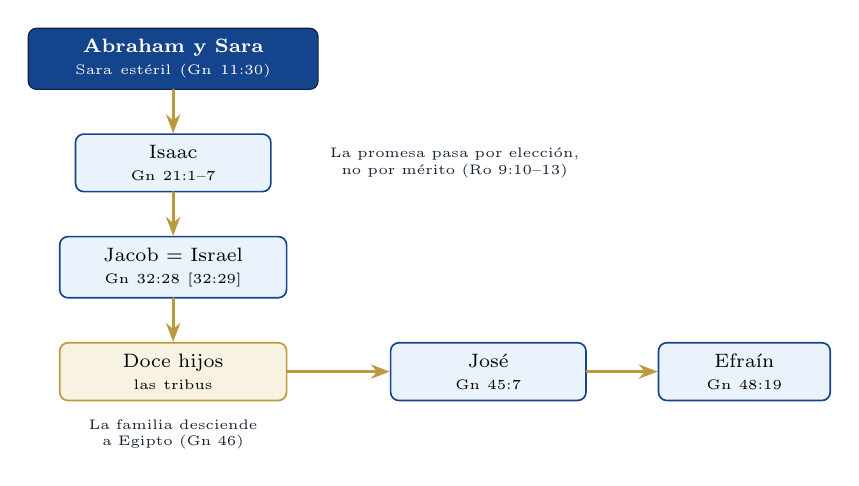
\begin{tikzpicture}[node distance=0.55cm]
\node[bloqueazul,text width=3.4cm] (ab) {Abraham y Sara\\{\tiny\mdseries Sara estéril (Gn 11:30)}};
\node[bloque,text width=2.2cm,below=of ab] (is) {Isaac\\{\tiny Gn 21:1--7}};
\begin{scope}[visible on=<2->]\node[bloque,text width=2.6cm,below=of is] (ja) {Jacob = Israel\\{\tiny Gn 32:28 [32:29]}};\end{scope}
\begin{scope}[visible on=<3->]\node[bloqueoro,text width=2.6cm,below=of ja] (do) {Doce hijos\\{\tiny las tribus}};\end{scope}
\begin{scope}[visible on=<4->]\node[bloque,text width=2.2cm,right=1.3cm of do] (jo) {José\\{\tiny Gn 45:7}};\end{scope}
\begin{scope}[visible on=<4->]\node[bloque,text width=1.9cm,right=0.9cm of jo] (ef) {Efraín\\{\tiny Gn 48:19}};\end{scope}
\begin{scope}[visible on=<4->]\draw[flecha] (ab) -- (is);\end{scope} \begin{scope}[visible on=<4->]\draw[flecha] (is) -- (ja);\end{scope} \begin{scope}[visible on=<4->]\draw[flecha] (ja) -- (do);\end{scope}
\begin{scope}[visible on=<4->]\draw[flecha] (do) -- (jo);\end{scope} \begin{scope}[visible on=<4->]\draw[flecha] (jo) -- (ef);\end{scope}
\begin{scope}[visible on=<5->]\node[etiq,text width=3.2cm,anchor=west] at ([xshift=0.6cm]is.east) {La promesa pasa por elección, no por mérito (Ro 9:10--13)};\end{scope}
\begin{scope}[visible on=<6->]\node[etiq,text width=3.2cm,below=3pt of do] {La familia desciende a Egipto (Gn 46)};\end{scope}
\end{tikzpicture}
\elabpropia
\end{frame}

\begin{frame}{José y el primer remanente}
\begin{cita}Dios me envió delante de vosotros para preservaros un \textbf{remanente} en la tierra y para daros vida por medio de una gran liberación.\fuente{(Gn 45:7)}\end{cita}
\centering
\begin{tikzpicture}[node distance=0.8cm]
\node[caja,text width=3.3cm,align=center] (a) {\textbf{Génesis}\\[2pt]\heb{שְׁאֵרִית} (\emph{she'erit})\\{\tiny Gn 45:7: la familia sobrevive}};
\begin{scope}[visible on=<2->]\node[caja,text width=3.3cm,align=center,right=of a] (b) {\textbf{Isaías}\\[2pt]\heb{שְׁאָר יָשׁוּב}\\{\tiny Is 10:20--22: «un remanente volverá»}};\end{scope}
\begin{scope}[visible on=<3->]\node[caja,text width=3.3cm,align=center,right=of b] (c) {\textbf{Pablo}\\[2pt]\grc{λεῖμμα κατ᾽ ἐκλογὴν χάριτος}\\{\tiny Ro 11:5: «remanente escogido por gracia»}};\end{scope}
\begin{scope}[visible on=<3->]\draw[-{Latex[length=2.5mm]},oro!90!ladrillo,line width=1.4pt] (a) -- (b);\end{scope}
\begin{scope}[visible on=<3->]\draw[-{Latex[length=2.5mm]},oro!90!ladrillo,line width=1.4pt] (b) -- (c);\end{scope}
\end{tikzpicture}
\elabpropia
\vspace{6pt}
\begin{clave}
Es la primera vez que \emph{she'erit} se aplica a la familia de Israel. Un remanente que sobrevive para que otros vivan: gracias a José come también «toda la tierra» (Gn 41:57).
\end{clave}
\end{frame}

\begin{frame}{Dios baja al exilio y promete visitar}
\centering{\large\heb{אָנֹכִי אֵרֵד עִמְּךָ מִצְרַיְמָה וְאָנֹכִי אַעַלְךָ גַם־עָלֹה}}\par\smallskip
\begin{cita}Yo descenderé contigo a Egipto, y yo también te haré subir de nuevo.\fuente{(Gn 46:4)}\end{cita}
\begin{tikzpicture}[node distance=0.32cm]
\node[bloqueazul,text width=2.05cm,font=\tiny\bfseries] (a) {Gn 50:24--25\\José: \heb{פָּקֹד יִפְקֹד}};
\begin{scope}[visible on=<2->]\node[bloque,text width=2.05cm,font=\tiny,right=of a] (b) {Éx 3:16\\Moisés: \heb{פָּקֹד פָּקַדְתִּי}};\end{scope}
\begin{scope}[visible on=<3->]\node[bloque,text width=2.05cm,font=\tiny,right=of b] (c) {Éx 13:19\\los huesos de José suben};\end{scope}
\begin{scope}[visible on=<4->]\node[bloque,text width=2.05cm,font=\tiny,right=of c] (d) {Heb 11:22\\un acto de fe};\end{scope}
\begin{scope}[visible on=<5->]\node[bloqueoro,text width=2.05cm,font=\tiny,right=of d] (e) {Lc 1:68\\«ha visitado y redimido»};\end{scope}
\begin{scope}[visible on=<5->]\draw[flecha] (a) -- (b);\end{scope} \begin{scope}[visible on=<5->]\draw[flecha] (b) -- (c);\end{scope} \begin{scope}[visible on=<5->]\draw[flecha] (c) -- (d);\end{scope} \begin{scope}[visible on=<5->]\draw[flecha] (d) -- (e);\end{scope}
\end{tikzpicture}
\elabpropia
\begin{notalam}[La fórmula de la visitación]
\emph{Paqod yifqod}, «Dios ciertamente os visitará», enlaza Génesis con Éxodo. Una tradición midrásica la entendió como la señal de redención transmitida desde José (Pirqé de-Rabí Eliézer 48).
\end{notalam}
\end{frame}

\begin{frame}{El Éxodo: Dios se acuerda}
\begin{columns}[T,onlytextwidth]
\begin{column}{0.46\textwidth}
\begin{cita}Y oyó Dios su gemido, y se acordó Dios de su pacto con Abraham, con Isaac y con Jacob.\fuente{(Éx 2:24)}\end{cita}
\begin{notalam}[\emph{Zajar}]
\heb{זָכַר}: actuar en favor de alguien por un compromiso, más que recordar un dato. Israel es \heb{בְּנִי בְכֹרִי}, «mi hijo, mi primogénito» (Éx 4:22).
\end{notalam}
\scriptsize Con Israel sale una «multitud mixta» (\heb{עֵרֶב רַב}, Éx 12:38, 48--49).
\end{column}
\begin{column}{0.50\textwidth}
\centering\textbf{\small\textcolor{cafe}{Los verbos de la redención (Éx 6:6--8)}}\par\smallskip
\begin{tikzpicture}[y=-0.66cm]
\foreach \i/\v/\h [count=\ovc,evaluate=\ovc as \ovk using int(\ovc+0)] in {0/Os sacaré/{וְהוֹצֵאתִי},1/Os libraré/{וְהִצַּלְתִּי},2/Os redimiré/{וְגָאַלְתִּי},3/Os tomaré por pueblo/{וְלָקַחְתִּי},4/Os introduciré en la tierra/{וְהֵבֵאתִי}}{\begin{scope}[visible on=<\ovk->]
  \node[caja,text width=4.6cm,minimum height=0.48cm,inner sep=2.5pt] at (0,\i) {\textbf{\v}\hfill\heb{\h}};\end{scope}}
\begin{scope}[visible on=<5->]\draw[decorate,decoration={brace,amplitude=4pt},sepia] (2.65,-0.25) -- (2.65,3.25) node[midway,right=4pt,font=\tiny,text width=0.9cm]{Pascua, mar, Sinaí};\end{scope}
\begin{scope}[visible on=<5->]\draw[decorate,decoration={brace,amplitude=4pt},sepia] (2.65,3.75) -- (2.65,4.25) node[midway,right=4pt,font=\tiny,text width=0.9cm]{Estudio 2};\end{scope}
\end{tikzpicture}
\elabpropia
\end{column}
\end{columns}
\end{frame}

% ===================================================
\section{Vocación}
\begin{frame}{Un pueblo sacerdotal}
\fotolado{panel_ex.jpg}{Elaboración propia: Éx 4:22 y 19:6 en texto hebreo consonántico (BHS).}
\begin{columns}[c,onlytextwidth]
\begin{column}{0.57\textwidth}
\begin{cita}Vosotros me seréis un reino de sacerdotes y una nación santa.\fuente{(Éx 19:6)}\end{cita}
\small \heb{מַמְלֶכֶת כֹּהֲנִים וְגוֹי קָדוֹשׁ}. Fórmula del Sinaí (Estudio 2), anticipada en los patriarcas:
\scriptsize
\begin{itemize}
\item \textbf{Altar}: Abraham invoca el nombre (Gn 12:7--8; 13:18).
\item \textbf{Intercesión}: por Sodoma y por Abimelec (Gn 18:22--33; 20:7).
\item \textbf{Enseñanza}: «justicia y juicio» a sus hijos (Gn 18:19).
\item \textbf{Preservar la vida}: José y la hambruna (Gn 41:57).
\item \textbf{Primogénito}: representa a los hermanos (Éx 4:22; Nm 3:12).
\end{itemize}
\end{column}
\begin{column}{0.41\textwidth}\end{column}
\end{columns}
\end{frame}

\begin{frame}{El llamamiento de Israel}
\centering
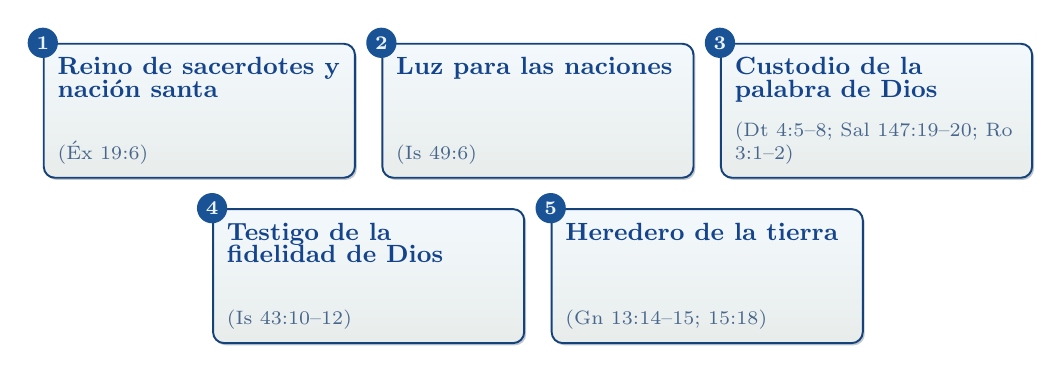
\begin{tikzpicture}
 \foreach \x/\y/\n/\t/\r in {0/0/1/{Reino de sacerdotes y nación santa}/{Éx 19:6},
    4.3/0/2/{Luz para las naciones}/{Is 49:6},
    8.6/0/3/{Custodio de la palabra de Dios}/{Dt 4:5--8; Sal 147:19--20; Ro 3:1--2},
    2.15/-2.1/4/{Testigo de la fidelidad de Dios}/{Is 43:10--12},
    6.45/-2.1/5/{Heredero de la tierra}/{Gn 13:14--15; 15:18}}{
  \node[caja,anchor=north] (b\n) at (\x,\y) {\parbox[t][1.35cm][t]{3.6cm}{\RaggedRight
    {\small\textbf{\textcolor{ladrillo}{\t}}}\par\vfill{\scriptsize\color{sepia}(\r)}}};
  \node[circle,fill=cafe,text=piedra,font=\scriptsize\bfseries,inner sep=1.6pt] at (b\n.north west) {\n};}
\end{tikzpicture}
\elabpropia
\vspace{4pt}
\begin{notalam}[El sacerdocio al final del camino]
Isaías sitúa el sacerdocio de Israel en el horizonte del regreso, «seréis llamados sacerdotes de YHWH» (Is 61:6), y lo abre a las naciones, de las cuales tomará «sacerdotes y levitas» (Is 66:21). Pedro aplica Éx 19:6 a los creyentes de la diáspora (1~P 2:9).
\end{notalam}
\end{frame}

% ===================================================
\section{Tradición judía}
\begin{frame}{Abraham en el midrash}
\small Relatos de la tradición, no crónica histórica: así leyó Israel su origen.\par\medskip
\centering
\begin{tikzpicture}
 \foreach \x/\n/\t/\d/\r in {0/1/{El rompedor de ídolos}/{Abram rompe las imágenes del taller de su padre Taré. Da forma narrativa a Jos 24:2.}/{Bereshit Rabbah 38:13},
   4.3/2/{«Abram el hebreo»}/{\heb{הָעִבְרִי} (\emph{ha-ivrí}) leído desde \emph{éver}, «el otro lado»: el mundo de un lado y Abram del otro.}/{Bereshit Rabbah 42:8},
   8.6/3/{Las diez pruebas}/{«Con diez pruebas fue probado Abraham, nuestro padre, y las superó todas».}/{Mishná, Avot 5:3}}{
  \node[caja,anchor=north] (b\n) at (\x,0) {\parbox[t][3.0cm][t]{3.6cm}{\RaggedRight
    {\small\textbf{\textcolor{ladrillo}{\t}}}\\[5pt]\small \d\par\vfill{\scriptsize\color{sepia}(\r)}}};
  \node[circle,fill=cafe,text=piedra,font=\scriptsize\bfseries,inner sep=1.6pt] at (b\n.north west) {\n};}
\end{tikzpicture}
\elabpropia
\vspace{4pt}
\begin{notalam}[Midrash y texto]
El relato de los ídolos es haggádico: pone en escena lo que Jos 24:2 deja implícito. Conviene distinguirlo del texto bíblico que lo inspira.
\end{notalam}
\end{frame}

\begin{frame}{Los padres en la oración diaria}
\centering{\large\heb{וְזוֹכֵר חַסְדֵי אָבוֹת וּמֵבִיא גּוֹאֵל לִבְנֵי בְנֵיהֶם}}\par\smallskip
\begin{cita}Dios de Abraham, Dios de Isaac y Dios de Jacob [\ldots] que se acuerda de las bondades de los padres y trae un redentor a los hijos de sus hijos.\fuente{(Amidá, bendición \emph{Avot})}\end{cita}
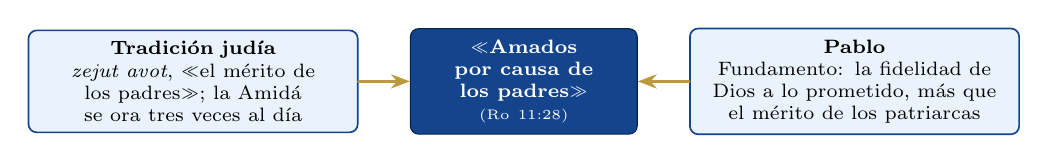
\begin{tikzpicture}
\node[bloque,text width=3.9cm,minimum height=1.25cm] (z) at (0,0) {\textbf{Tradición judía}\\\emph{zejut avot}, «el mérito de los padres»; la Amidá se ora tres veces al día};
\begin{scope}[visible on=<2->]\node[bloque,text width=3.9cm,minimum height=1.25cm] (p) at (8.4,0) {\textbf{Pablo}\\Fundamento: la fidelidad de Dios a lo prometido, más que el mérito de los patriarcas};\end{scope}
\begin{scope}[visible on=<3->]\node[bloqueazul,text width=2.6cm] (c) at (4.2,0) {«Amados por causa de los padres»\\{\tiny\mdseries (Ro 11:28)}};\end{scope}
\begin{scope}[visible on=<3->]\draw[flecha] (z) -- (c);\end{scope} \begin{scope}[visible on=<3->]\draw[flecha] (p) -- (c);\end{scope}
\end{tikzpicture}
\elabpropia
\end{frame}

\begin{frame}{Pésaj: cuatro copas y una quinta}
\begin{columns}[T,onlytextwidth]
\begin{column}{0.56\textwidth}
\centering
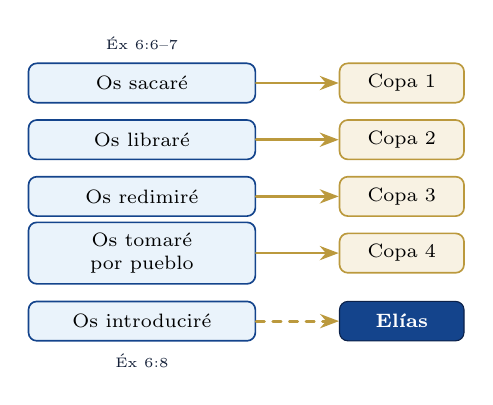
\begin{tikzpicture}[y=-0.72cm]
\foreach \i/\v [count=\ovc,evaluate=\ovc as \ovk using int(\ovc+0)] in {0/Os sacaré,1/Os libraré,2/Os redimiré,3/Os tomaré por pueblo}{\begin{scope}[visible on=<\ovk->]
  \node[bloque,text width=2.6cm,minimum height=0.5cm] (v\i) at (0,\i) {\v};
  \node[bloqueoro,text width=1.3cm,minimum height=0.5cm] (c\i) at (3.3,\i) {Copa \the\numexpr\i+1\relax};
  \draw[flecha] (v\i) -- (c\i);\end{scope}}
\begin{scope}[visible on=<4->]\node[bloque,text width=2.6cm,minimum height=0.5cm] (v4) at (0,4.2) {Os introduciré};\end{scope}
\begin{scope}[visible on=<4->]\node[bloqueazul,text width=1.3cm,minimum height=0.5cm] (c4) at (3.3,4.2) {Elías};\end{scope}
\begin{scope}[visible on=<4->]\draw[flecha,dashed] (v4) -- (c4);\end{scope}
\begin{scope}[visible on=<4->]\node[etiq,above=1pt of v0] {Éx 6:6--7};\end{scope}
\begin{scope}[visible on=<4->]\node[etiq,below=1pt of v4] {Éx 6:8};\end{scope}
\end{tikzpicture}
\notafig{Elaboración propia a partir de Talmud de Jerusalén, Pesajim 10:1 (Neusner, 1982--1994).}
\end{column}
\begin{column}{0.40\textwidth}\small
«En cada generación, cada uno debe verse como si hubiera salido de Egipto» (Mishná, Pesajim 10:5).\par\medskip
\begin{notalam}[La copa de Elías]
La quinta expresión quedó ligada en la costumbre posterior a la copa de Elías, el profeta que anuncia la redención futura. La mesa se cierra con «el año próximo en Jerusalén».
\end{notalam}
\end{column}
\end{columns}
\end{frame}

\begin{frame}{Memoria que se vuelve esperanza}
\begin{columns}[T,onlytextwidth]
\begin{column}{0.48\textwidth}\small
\textbf{\textcolor{ladrillo}{Rosh Hashaná}}\par\smallskip
Se leen Gn 21--22 y se toca un cuerno de carnero: «para que me acuerde de vosotros de la atadura de Isaac» (Talmud, Rosh Hashaná 16a).\par\medskip
\begin{clave}
La Akedá quedó unida, en la liturgia, al juicio de Dios y a su memoria compasiva.
\end{clave}
\end{column}
\begin{column}{0.48\textwidth}\small
\textbf{\textcolor{ladrillo}{La Shejiná en el exilio}}\par\smallskip
«A todo lugar adonde fueron desterrados, la Shejiná fue con ellos: a Egipto [\ldots], a Babilonia» (Talmud, Meguilá 29a). Desarrolla Gn 46:4.\par\medskip
\begin{notalam}[Ezequiel junto al Quebar]
La enseñanza pone en una sola línea el exilio de Egipto y el de Babilonia; Ezequiel oye que Dios será para los desterrados «un pequeño santuario» (Ez 11:16).
\end{notalam}
\end{column}
\end{columns}
\end{frame}

% ===================================================
\section{Restauración}
\begin{frame}{El patrón en la Torá}
\centering\footnotesize\renewcommand{\arraystretch}{1.25}
\begin{tabular}{>{\RaggedRight\arraybackslash}p{2.0cm}>{\RaggedRight\arraybackslash}p{4.9cm}>{\RaggedRight\arraybackslash}p{4.7cm}}
\toprule
{\leavevmode\color{ladrillo}\bfseries Texto} & {\leavevmode\color{ladrillo}\bfseries Promesa} & {\leavevmode\color{ladrillo}\bfseries Proyección}\\\midrule
Gn 15:13--16 & Destierro, juicio al opresor, regreso & Dt 30:1--5; Jer 29:10--14\\
Gn 17:7 & Pacto perpetuo con la descendencia & Jer 31:35--37 [31:34--36]; Ro 11:29\\
Gn 45:7 & Un remanente preservado & Is 10:20--22; Ro 11:5\\
Gn 46:4 & Dios baja al exilio y hace subir & Is 43:2; Ez 11:16\\
Gn 50:24 & «Dios ciertamente os visitará» & Éx 3:16; Lc 1:68\\
Éx 2:24 & Dios se acuerda del pacto & Lv 26:42--45; Lc 1:72--73\\
Éx 6:6--8 & Sacar, librar, redimir, tomar, introducir & Is 43:1; Jer 16:14--15\\
\bottomrule
\end{tabular}
\elabpropia
\end{frame}

\begin{frame}{Lv 26:42: la memoria en orden invertido}
\begin{cita}Me acordaré de mi pacto con Jacob, y también de mi pacto con Isaac, y también de mi pacto con Abraham me acordaré, y de la tierra me acordaré.\fuente{(Lv 26:42)}\end{cita}
\centering
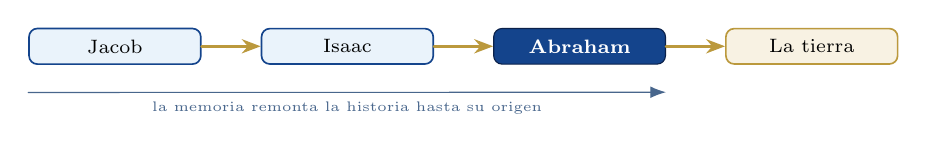
\begin{tikzpicture}[node distance=0.75cm]
\node[bloque,text width=1.9cm] (j) {Jacob};
\begin{scope}[visible on=<2->]\node[bloque,text width=1.9cm,right=of j] (i) {Isaac};\end{scope}
\begin{scope}[visible on=<3->]\node[bloqueazul,text width=1.9cm,right=of i] (a) {Abraham};\end{scope}
\begin{scope}[visible on=<4->]\node[bloqueoro,text width=1.9cm,right=of a] (t) {La tierra};\end{scope}
\begin{scope}[visible on=<4->]\draw[flecha] (j) -- (i);\end{scope} \begin{scope}[visible on=<4->]\draw[flecha] (i) -- (a);\end{scope} \begin{scope}[visible on=<4->]\draw[flecha] (a) -- (t);\end{scope}
\begin{scope}[visible on=<4->]\draw[sepia,-{Latex[length=2mm]}] ([yshift=-0.35cm]j.south west) -- node[below,etiq,text=sepia]{la memoria remonta la historia hasta su origen} ([yshift=-0.35cm]a.south east);\end{scope}
\end{tikzpicture}
\elabpropia
\vspace{8pt}
\begin{clave}
El regreso descansa en el pacto con los padres, no en el mérito de la generación desterrada. En la Torá ningún texto es tan explícito como Lv 26.
\end{clave}
\end{frame}

\begin{frame}{Isaías: mirad la roca}
\fotolado{panel_is51.jpg}{Elaboración propia: Is 51:2 en texto hebreo consonántico (BHS).}
\begin{columns}[c,onlytextwidth]
\begin{column}{0.57\textwidth}
\begin{cita}Mirad a Abraham vuestro padre y a Sara que os dio a luz; porque era uno solo cuando lo llamé, y lo bendije y lo multipliqué. Ciertamente consolará YHWH a Sion.\fuente{(Is 51:2--3)}\end{cita}
\scriptsize
\begin{itemize}
\item \textbf{El origen como garantía}: quien hizo una nación de uno solo puede rehacer a Sion.
\item \textbf{Is 41:8--9}: «descendencia de Abraham mi amigo [\ldots] te escogí y no te deseché».
\item \textbf{Is 43:19}: \heb{הִנְנִי עֹשֶׂה חֲדָשָׁה}, «hago una cosa nueva»: el nuevo éxodo.
\item \textbf{Is 11:11, 16}: el Señor extenderá su mano «por segunda vez» (\heb{שֵׁנִית}), como cuando Israel subió de Egipto.
\end{itemize}
\end{column}
\begin{column}{0.41\textwidth}\end{column}
\end{columns}
\end{frame}

\begin{frame}{Jeremías: un pacto tan firme como el cosmos}
\begin{columns}[T,onlytextwidth]
\begin{column}{0.48\textwidth}
\centering\textbf{\small\textcolor{cafe}{La fórmula de juramento cambia (Jer 16:14--15)}}\par\medskip
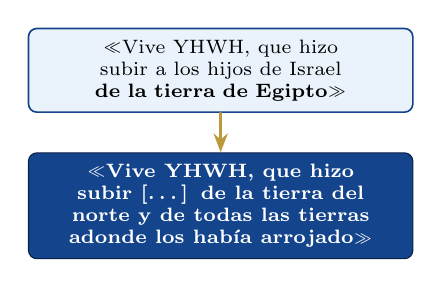
\begin{tikzpicture}[node distance=0.5cm]
\node[bloque,text width=4.6cm] (a) {«Vive YHWH, que hizo subir a los hijos de Israel \textbf{de la tierra de Egipto}»};
\begin{scope}[visible on=<2->]\node[bloqueazul,text width=4.6cm,below=of a] (b) {«Vive YHWH, que hizo subir [\ldots] \textbf{de la tierra del norte} y de todas las tierras adonde los había arrojado»};\end{scope}
\begin{scope}[visible on=<2->]\draw[flecha] (a) -- (b);\end{scope}
\end{tikzpicture}
\elabpropia
\vspace{2pt}
{\scriptsize\textbf{Jer 31:9 [31:8]}: «soy a Israel por padre, y Efraín es mi primogénito» (cf. Éx 4:22).}
\end{column}
\begin{column}{0.48\textwidth}
\begin{cita}Si faltaren estas leyes delante de mí, dice YHWH, también la descendencia de Israel faltará para no ser nación delante de mí para siempre.\fuente{(Jer 31:36 [31:35])}\end{cita}
\begin{cita}[fontupper=\scriptsize\itshape]Si no permanece mi pacto con el día y la noche [\ldots], también desecharé la descendencia de Jacob [\ldots]. Porque haré volver a sus cautivos y tendré de ellos misericordia.\fuente{(Jer 33:25--26)}\end{cita}
\end{column}
\end{columns}
\end{frame}

\begin{frame}{Miqueas y Lucas: el juramento a los padres}
\centering{\large\heb{תִּתֵּן אֱמֶת לְיַעֲקֹב חֶסֶד לְאַבְרָהָם}}\par\smallskip
\begin{cita}Darás fidelidad a Jacob, y misericordia a Abraham, como lo juraste a nuestros padres desde los días antiguos.\fuente{(Mi 7:20)}\end{cita}
\begin{columns}[T,onlytextwidth]
\begin{column}{0.48\textwidth}
\begin{cita}[fontupper=\scriptsize\itshape]Socorrió a Israel su siervo, acordándose de la misericordia, como habló a nuestros padres, a Abraham y a su descendencia para siempre.\fuente{(Lc 1:54--55)}\end{cita}
\end{column}
\begin{column}{0.48\textwidth}
\begin{cita}[fontupper=\scriptsize\itshape]Ha visitado y redimido a su pueblo [\ldots] para acordarse de su santo pacto, del juramento que hizo a Abraham nuestro padre.\fuente{(Lc 1:68, 72--73)}\end{cita}
\end{column}
\end{columns}
\begin{clave}
Los verbos son los del Éxodo: visitar, redimir, acordarse. Lucas presenta la venida del Mesías como cumplimiento del pacto abrahámico.
\end{clave}
\end{frame}

\begin{frame}{Pablo: Ro 11:28--29}
\fotolado{panel_gal38.jpg}{Elaboración propia: Gá 3:8 en escritura uncial (texto NA28).}
\begin{columns}[c,onlytextwidth]
\begin{column}{0.57\textwidth}
\begin{cita}En cuanto a la elección, son amados por causa de los padres; porque irrevocables son los dones y el llamamiento de Dios.\fuente{(Ro 11:28--29)}\end{cita}
\scriptsize
\begin{itemize}
\setlength{\itemsep}{0pt}
\item \grc{ἀμεταμέλητα}: «sin arrepentimiento»; promesa sin vuelta atrás.
\item \textbf{Gá 3:8}: la promesa a Abraham es «evangelio anunciado de antemano».
\item \textbf{Ro 4:17}: Abraham, padre de los creyentes de las naciones.
\item \textbf{Ro 15:8}: Cristo vino «para confirmar las promesas hechas a los padres».
\end{itemize}
\begin{notalam}[¿Quién es la raíz? (Ro 11:16)]
Muchos comentaristas la identifican con los patriarcas (Moo, 1996); otros, con Cristo o con el remanente creyente.
\end{notalam}
\end{column}
\begin{column}{0.41\textwidth}\end{column}
\end{columns}
\end{frame}

% ===================================================
\section{Síntesis}
\begin{frame}{Síntesis}
\begin{tcolorbox}[colback=piedra,colframe=ladrillo,boxrule=1pt,arc=3pt,fontupper=\small]
\textbf{\textcolor{cafe}{Israel en su origen:}} un pueblo nacido de una pareja estéril, llamado a bendecir a las naciones y sostenido por un pacto perpetuo que anuncia de antemano destierro y regreso. Por ese pacto Dios «se acordó» en Egipto (Éx 2:24); ese pacto sostiene el nuevo éxodo de Isaías y Jeremías, y permite a Pablo decir que Israel sigue siendo «amado por causa de los padres» (Ro 11:28).
\end{tcolorbox}
\scriptsize\renewcommand{\arraystretch}{1.25}
\begin{tabular}{>{\RaggedRight\arraybackslash}p{3.0cm}>{\RaggedRight\arraybackslash}p{8.6cm}}
\toprule
{\leavevmode\color{ladrillo}\bfseries Eje} & {\leavevmode\color{ladrillo}\bfseries Lo que deja esta etapa}\\\midrule
Creación de Dios & Sara estéril, Isaac hijo de la promesa (Gn 11:30; 21:1--7; Is 51:1--3)\\
Vocación sacerdotal & Bendición para las naciones; altar, intercesión, enseñanza, primogenitura\\
Restauración & Gn 15:13--16; 46:4; 50:24; Éx 2:24; Lv 26:42\\
Proyección & Isaías (nuevo éxodo), Jeremías (pacto como el cosmos), Pablo (Ro 11:28--29)\\
\bottomrule
\end{tabular}
\elabpropia
\end{frame}

\begin{frame}{Hacia el Estudio 2}
\begin{columns}[c,onlytextwidth]
\begin{column}{0.55\textwidth}
\begin{cita}Vosotros visteis lo que hice a los egipcios, y cómo os tomé sobre alas de águila y os he traído a mí.\fuente{(Éx 19:4)}\end{cita}
\small El Éxodo no se detiene en el mar. En el Sinaí, lo que aquí está en germen tomará forma de \destacar{pacto}, \destacar{ley} y \destacar{santuario}.
\end{column}
\begin{column}{0.42\textwidth}
\begin{tcolorbox}[colback=cafe,colframe=cafeosc,coltext=piedra,boxrule=0.8pt,arc=3pt,fontupper=\small]
\textbf{Estudio 2}\par\smallskip
Del Éxodo a la muerte de Josué: Sinaí, tabernáculo, desierto, conquista y reparto de la tierra.
\end{tcolorbox}
\end{column}
\end{columns}
\end{frame}

% ===================================================
\section{Reflexión}
\begin{frame}{Para la reflexión}
\begin{enumerate}\setlength{\itemsep}{10pt}
\item Isaías invita a «mirar la roca de donde fuisteis tallados» (Is 51:1). ¿Cómo cambia la lectura al recordar que Israel nació de una mujer estéril?
\item Gn 15 anuncia el sufrimiento de Israel antes de que exista. ¿Qué dice esto sobre la relación entre los juicios de Dios y su fidelidad?
\item Si Abraham fue llamado a ser bendición para las naciones, ¿qué responsabilidad tienen hoy los creyentes de las naciones hacia Israel (Ro 11:18; 15:27)?
\item ¿En qué se parecen y en qué se diferencian el \emph{zejut avot} rabínico y la afirmación de Pablo en Ro 11:28?
\end{enumerate}
\end{frame}

% ===================================================
\section{Glosario}
\begin{frame}{Glosario}
\begin{columns}[T,onlytextwidth]
\begin{column}{0.48\textwidth}\footnotesize
\textbf{Akedá} (\heb{עֲקֵדָה}): «atadura»; relato de Gn 22.\par\smallskip
\textbf{Berit} (\heb{בְּרִית}): pacto; \emph{berit olam}, pacto perpetuo.\par\smallskip
\textbf{Berit bein ha-betarim}: «pacto entre las piezas» (Gn 15).\par\smallskip
\textbf{Bejor} (\heb{בְּכוֹר}): primogénito (Éx 4:22; Jer 31:9).\par\smallskip
\textbf{Emuná} (\heb{אֱמוּנָה}): firmeza, fidelidad, fe.\par\smallskip
\textbf{Érev rav} (\heb{עֵרֶב רַב}): multitud mixta (Éx 12:38).\par\smallskip
\textbf{Ha-ivrí} (\heb{הָעִבְרִי}): «el hebreo» (Gn 14:13).
\end{column}
\begin{column}{0.48\textwidth}\footnotesize
\textbf{Mamléjet kohaním} (\heb{מַמְלֶכֶת כֹּהֲנִים}): reino de sacerdotes (Éx 19:6).\par\smallskip
\textbf{Paqad} (\heb{פָּקַד}): visitar, intervenir a favor (Gn 50:24).\par\smallskip
\textbf{She'erit} (\heb{שְׁאֵרִית}): remanente (Gn 45:7).\par\smallskip
\textbf{Shejiná} (\heb{שְׁכִינָה}): presencia de Dios con su pueblo (término rabínico).\par\smallskip
\textbf{Shuv} (\heb{שׁוּב}): volver; regreso y arrepentimiento.\par\smallskip
\textbf{Zajar} (\heb{זָכַר}): acordarse, actuar en virtud de un compromiso.\par\smallskip
\textbf{Zejut avot} (\heb{זְכוּת אָבוֹת}): mérito de los padres.
\end{column}
\end{columns}
\end{frame}

% ===================================================
\section{Referencias}
\begin{frame}[allowframebreaks]{Referencias}
\tiny
\refapa{Albright, W.~F. (1954). Northwest-Semitic names in a list of Egyptian slaves from the eighteenth century B.C. \emph{Journal of the American Oriental Society, 74}(4), 222--233.}
\refapa{\emph{Biblia Hebraica Stuttgartensia} (5.ª ed.). (1997). Deutsche Bibelgesellschaft.}
\refapa{Bietak, M. (1996). \emph{Avaris: The capital of the Hyksos}. British Museum Press.}
\refapa{Danby, H. (Trad.). (1933). \emph{The Mishnah}. Oxford University Press.}
\refapa{Epstein, I. (Ed.). (1935--1948). \emph{The Babylonian Talmud}. Soncino Press.}
\refapa{Freedman, H., \& Simon, M. (Eds.). (1939). \emph{Midrash Rabbah}. Soncino Press.}
\refapa{Friedlander, G. (Trad.). (1916). \emph{Pirkê de Rabbi Eliezer}. Kegan Paul.}
\refapa{Guggenheimer, H.~W. (1998). \emph{Seder Olam: The rabbinic view of biblical chronology}. Jason Aronson.}
\refapa{Hayes, W.~C. (1955). \emph{A papyrus of the late Middle Kingdom in the Brooklyn Museum}. Brooklyn Museum.}
\refapa{Hays, R.~B. (1989). \emph{Echoes of Scripture in the letters of Paul}. Yale University Press.}
\refapa{Hoffmeier, J.~K. (1997). \emph{Israel in Egypt: The evidence for the authenticity of the Exodus tradition}. Oxford University Press.}
\refapa{Josefo, F. (1987). \emph{The works of Josephus} (W. Whiston, Trad.). Hendrickson.}
\refapa{Kitchen, K.~A. (2003). \emph{On the reliability of the Old Testament}. Eerdmans.}
\refapa{Moo, D.~J. (1996). \emph{The epistle to the Romans}. Eerdmans.}
\refapa{Neusner, J. (Trad.). (1982--1994). \emph{The Talmud of the Land of Israel}. University of Chicago Press.}
\refapa{Newberry, P.~E. (1893). \emph{Beni Hasan} (Parte I). Egypt Exploration Fund.}
\refapa{\emph{Novum Testamentum Graece} (28.ª ed.). (2012). Deutsche Bibelgesellschaft.}
\refapa{ONE FOR ISRAEL Ministry. (2025, 3 de julio). \emph{What does «all Israel will be saved» mean in Romans 11?} \url{https://www.oneforisrael.org/what-does-all-israel-will-be-saved-mean-in-romans-11/}}
\refapa{Rahlfs, A., \& Hanhart, R. (Eds.). (2006). \emph{Septuaginta} (ed. rev.). Deutsche Bibelgesellschaft.}
\refapa{Sacks, J. (Trad.). (2009). \emph{The Koren Siddur}. Koren Publishers.}
\refapa{Sapir-Hen, L., \& Ben-Yosef, E. (2013). The introduction of domestic camels to the southern Levant: Evidence from the Aravah Valley. \emph{Tel Aviv, 40}(2), 277--285.}
\refapa{Sarna, N.~M. (1989). \emph{Genesis} (The JPS Torah Commentary). Jewish Publication Society.}
\refapa{Sarna, N.~M. (1991). \emph{Exodus} (The JPS Torah Commentary). Jewish Publication Society.}
\refapa{Thompson, T.~L. (1974). \emph{The historicity of the patriarchal narratives}. De Gruyter.}
\refapa{Van Seters, J. (1975). \emph{Abraham in history and tradition}. Yale University Press.}
\refapa{Wright, N.~T. (2013). \emph{Paul and the faithfulness of God}. Fortress Press.}
\end{frame}
\end{document}
